\documentclass[11pt,a4paper]{article}

\usepackage[utf8]{inputenc}
\usepackage[T1]{fontenc}
\usepackage[brazil]{babel}
\usepackage{amsmath, amssymb}
\usepackage{graphicx}
\usepackage{booktabs}
\usepackage{listings}
\usepackage{xcolor}
\usepackage{geometry}
\usepackage{caption}
\usepackage[hidelinks]{hyperref}
\geometry{margin=2.5cm}

\graphicspath{{../analise/figuras/}}

\lstset{
  basicstyle=\ttfamily\footnotesize,
  breaklines=true,
  frame=single,
  columns=fullflexible,
  keepspaces=true
}

\title{\textbf{Otimização de Telemetria com Buffer Circular}\\[4pt]
\large Comparação entre alocação dinâmica O(n) e buffer circular O(1)\\
em uma arquitetura cliente--servidor com MQTT}
\author{Silvio Fittipaldi \and Bernardo Heuer \and Rodrigo Nunes}
\date{\today}

\begin{document}
\maketitle

\begin{abstract}
Este trabalho compara duas estratégias de gerência de memória para um fluxo de
telemetria de alta frequência: uma estrutura de \emph{alocação dinâmica}
(anti-padrão, custo $O(n)$ por inserção) e um \emph{buffer circular} com índices
\texttt{head}/\texttt{tail} e operações $O(1)$. O enunciado original é embarcado
(ESP32); aqui ele é reproduzido em uma arquitetura cliente--servidor de software,
preservando todos os objetivos didáticos: duas vertentes comparadas, transmissão
MQTT, modelo produtor--consumidor, instrumentação de tempo e memória, testes de
escala ($N = 100/5.000/20.000/100.000$), painel com gráficos de dados e de
performance, e a presente análise. Os resultados confirmam empiricamente o
contraste assintótico esperado e evidenciam o impacto da instabilidade de rede.
\end{abstract}

\section{Introdução e adaptação}

O problema clássico de telemetria embarcada expõe uma disparidade temporal: a
captura de sensores ocorre na escala de microssegundos, enquanto a transmissão
em rede ocorre na escala de milissegundos. Se o produtor de dados ficar acoplado
ao consumidor de rede, a amostragem é estrangulada pela latência da rede; pior,
se a estrutura que acumula amostras crescer ou se reorganizar a cada inserção, o
custo de CPU e de memória degrada de forma super-linear.

Como o ambiente de execução não dispõe de hardware embarcado, o ESP32 foi
substituído por um \textbf{cliente em C++17} que gera amostras simuladas em alta
frequência. A equivalência entre o enunciado e esta versão está na
Tabela~\ref{tab:equiv}.

\begin{table}[h]
\centering
\caption{Equivalência entre o enunciado embarcado e a versão cliente--servidor.}
\label{tab:equiv}
\small
\begin{tabular}{@{}ll@{}}
\toprule
\textbf{Conceito (embarcado)} & \textbf{Equivalente (cliente--servidor)} \\
\midrule
ESP32 capturando sensor & Cliente produtor em C++ (amostras simuladas) \\
Captura ($\mu$s) $\times$ rede (ms) & Geração em memória ($\mu$s) $\times$ publicação MQTT (ms) \\
Transmissão MQTT & Mantida: publicação em broker Mosquitto \\
\texttt{micros()} & \texttt{QueryPerformanceCounter} / \texttt{steady\_clock} ($\mu$s/ns) \\
\texttt{ESP.getFreeHeap()} / fragmentação & Contadores globais de \texttt{new}/\texttt{delete} + RSS do SO \\
Colapso por \emph{stack overflow} & Crescimento ilimitado de memória / risco de OOM \\
Serial Plotter & Dashboard web (Node-RED) \\
\bottomrule
\end{tabular}
\end{table}

O servidor é composto pelo broker Eclipse Mosquitto~\cite{mosquitto} e pelo
dashboard Node-RED~\cite{nodered}, ambos em contêineres Docker, comunicando-se
pelo protocolo MQTT~\cite{mqtt311}.

\paragraph{Adaptações de ambiente.} Duas escolhas de engenharia, no mesmo espírito
da adaptação acima, tornaram o projeto autossuficiente: (i) a camada MQTT foi
implementada como um cliente MQTT 3.1.1~\cite{mqtt311} mínimo sobre \emph{sockets}
TCP (Winsock/BSD), preservando o contrato \texttt{publishSync} (bloqueante) versus
\texttt{publishAsync} (não bloqueante) sem depender de bibliotecas externas como o
Eclipse Paho~\cite{paho}; e (ii) o \emph{build} usa \texttt{g++} diretamente, além
de um \texttt{CMakeLists.txt} canônico. Nenhuma dessas escolhas altera os objetivos
didáticos.

\section{As duas vertentes}

\paragraph{Vertente 1 --- \texttt{DynamicBuffer} (anti-padrão, $O(n)$).}
Reproduz explicitamente o problema. Em duas sub-variantes:
\begin{itemize}
  \item \textbf{SHIFT}: mantém uma janela de tamanho $W$; ao encher, remove o
  primeiro elemento deslocando todos os demais (\texttt{erase(begin)}), custo
  $\Theta(W)$ por inserção.
  \item \textbf{REALLOC}: \emph{realloc} manual a cada amostra --- aloca um bloco
  com uma posição a mais, copia todo o conteúdo e libera o anterior. Custo $O(n)$
  por inserção, crescimento ilimitado e $N$ alocações.
\end{itemize}

\paragraph{Vertente 2 --- \texttt{RingBuffer} (eficiente, $O(1)$).}
Classe própria com \texttt{head}/\texttt{tail} e \texttt{count}; aloca o
armazenamento \textbf{uma única vez} no construtor e nunca realoca. As operações
usam apenas aritmética modular ($\texttt{idx} = (\texttt{idx}+1) \bmod
\texttt{cap}$): não há \texttt{erase}, \texttt{insert(begin)}, \texttt{memmove}
nem \texttt{realloc}. Política de \emph{overflow}: sobrescrever o mais antigo
(telemetria prioriza dados recentes).

\section{Análise Assintótica}

A análise abaixo emprega a notação assintótica padrão~\cite{cormen2009}.

\paragraph{Vertente 1 (SHIFT).} A inserção com manutenção de janela executa um
\texttt{push\_back} amortizado $O(1)$ seguido, quando a janela está cheia, de um
deslocamento de $W-1$ elementos. Logo o custo por inserção é $\Theta(W)$ e o
custo total de $N$ inserções é
\[
T_{\text{shift}}(N) \;=\; \Theta(N \cdot W).
\]

\paragraph{Vertente 1 (REALLOC).} A $i$-ésima inserção copia os $i-1$ elementos
já existentes mais um, ou seja, $\Theta(i)$. O custo total é
\[
T_{\text{realloc}}(N) \;=\; \sum_{i=1}^{N} \Theta(i)
\;=\; \Theta\!\left(\frac{N(N+1)}{2}\right) \;=\; \Theta(N^2),
\]
e o número de alocações é exatamente $N$, com pico de bytes vivos proporcional a
$N \cdot \texttt{sizeof(Sample)}$.

\paragraph{Vertente 2 (RingBuffer).} Cada \texttt{push} e cada \texttt{pop} fazem
trabalho constante (escrita/leitura mais incremento modular):
\[
T_{\text{ring}}(N) \;=\; \Theta(N), \qquad \text{com } 1 \text{ alocação total.}
\]
O dreno em lote de $k$ itens (\texttt{popBatch}) custa $\Theta(k)$, somando
$\Theta(N)$ ao longo da execução.

A Figura~\ref{fig:lat} confirma o contraste: a latência média de inserção da
Vertente 1 cresce com $N$/$W$, enquanto a da Vertente 2 permanece praticamente
constante (no piso de resolução do relógio de alta precisão~\cite{cppref_chrono}). A Figura~\ref{fig:dist} mostra a
distribuição completa por inserção, e a Figura~\ref{fig:jitter} mostra o
\emph{jitter} (desvio-padrão da latência), também maior na vertente $O(n)$.

\begin{figure}[h]
\centering
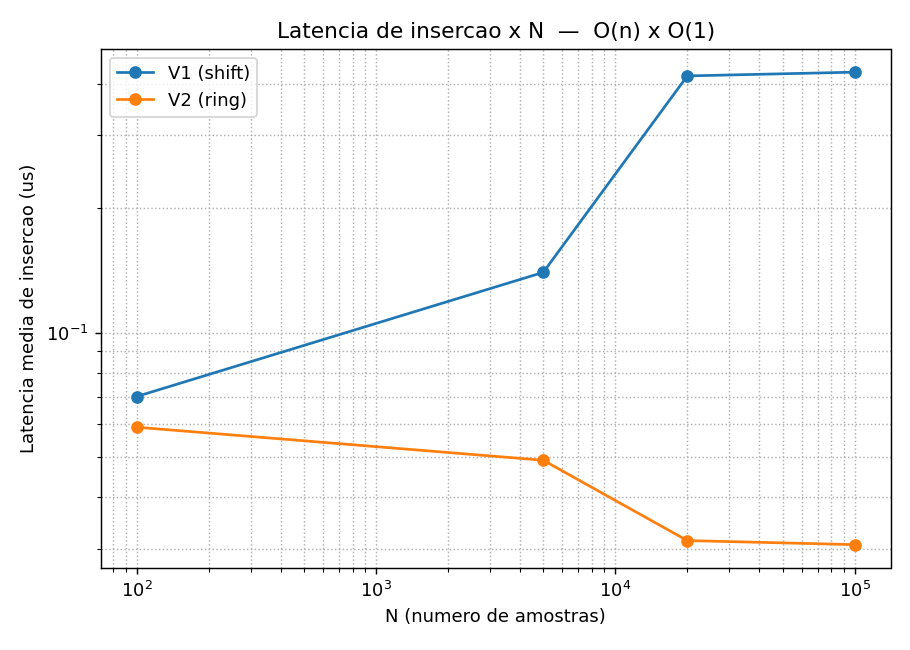
\includegraphics[width=0.78\textwidth]{fig_latencia_vs_N.png}
\caption{Latência média de inserção em função de $N$ (eixos log--log). A Vertente~1
(\texttt{shift}, $O(n)$) cresce; a Vertente~2 (\texttt{ring}, $O(1)$) é plana.}
\label{fig:lat}
\end{figure}

\begin{figure}[h]
\centering
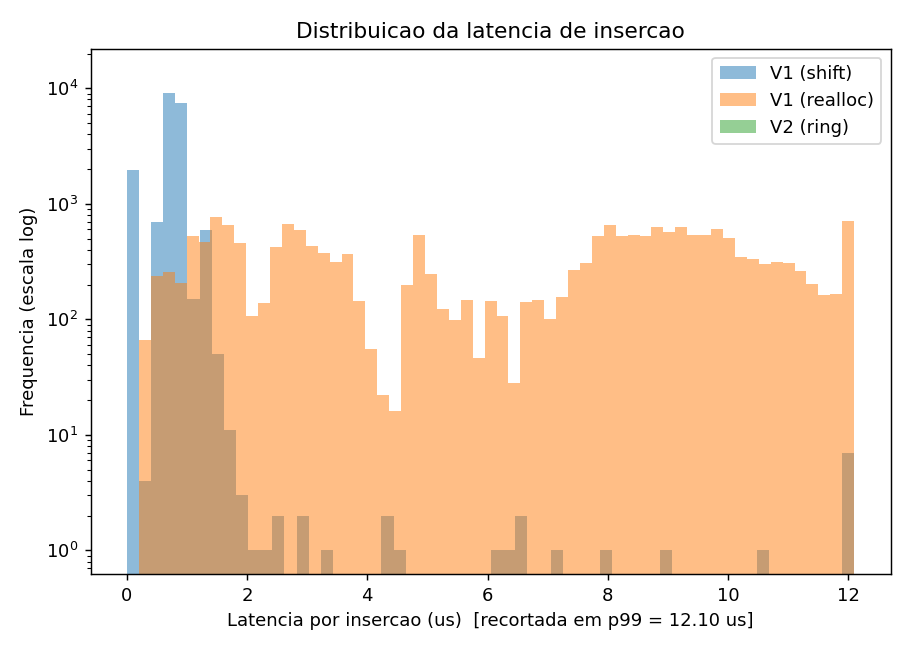
\includegraphics[width=0.78\textwidth]{fig_dist_latencia.png}
\caption{Distribuição da latência por inserção. A cauda longa da variante
\texttt{realloc} reflete as cópias de arrays cada vez maiores.}
\label{fig:dist}
\end{figure}

\begin{figure}[h]
\centering
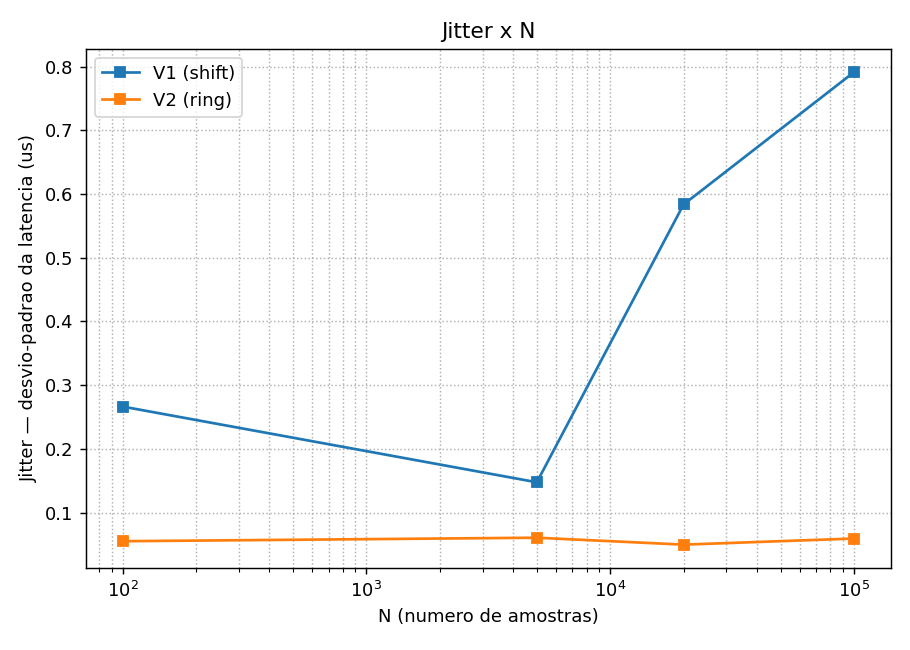
\includegraphics[width=0.78\textwidth]{fig_jitter_vs_N.png}
\caption{Jitter (desvio-padrão da latência de inserção) em função de $N$.}
\label{fig:jitter}
\end{figure}

\section{Diagnóstico de Memória}

A métrica primária de memória --- portável entre sistemas operacionais --- são os
\textbf{contadores globais de \texttt{operator new}/\texttt{delete}}, que
interceptam toda alocação dinâmica do processo e atribuem à estrutura de dados
apenas as alocações ocorridas durante suas inserções (isolando MQTT e
\emph{setup}). De forma complementar, registra-se o pico de RSS do processo.

A Tabela~\ref{tab:mem} resume os valores medidos. A Vertente~2 faz \textbf{uma}
alocação para $N$ até $100.000$, com volume constante. A variante \texttt{realloc}
da Vertente~1 faz $N$ alocações e acumula bytes em ritmo quadrático --- chegando a
$\sim 4{,}8$\,GB de bytes solicitados em $N=20.000$ ---, evidência direta da
fragmentação e do crescimento que, no contexto embarcado, levariam ao colapso por
falta de memória. As Figuras~\ref{fig:mem} e~\ref{fig:bytes} ilustram o
crescimento.

\begin{table}[h]
\centering
\caption{Diagnóstico de memória (valores representativos medidos). \texttt{n\_allocs}
e \texttt{alloc\_bytes} referem-se à estrutura de dados.}
\label{tab:mem}
\small
\begin{tabular}{@{}lrrr@{}}
\toprule
\textbf{Configuração} & \textbf{N} & \textbf{n\_allocs} & \textbf{alloc\_bytes} \\
\midrule
V2 \texttt{ring}    & 100.000 & 1 ou 2 & $\approx 98$\,KB (constante) \\
V1 \texttt{shift}   & 100.000 & 12     & $\approx 98$\,KB \\
V1 \texttt{realloc} & 5.000   & 5.000  & $\approx 300$\,MB \\
V1 \texttt{realloc} & 20.000  & 20.000 & $\approx 4{,}8$\,GB \\
\bottomrule
\end{tabular}
\end{table}

\begin{figure}[h]
\centering
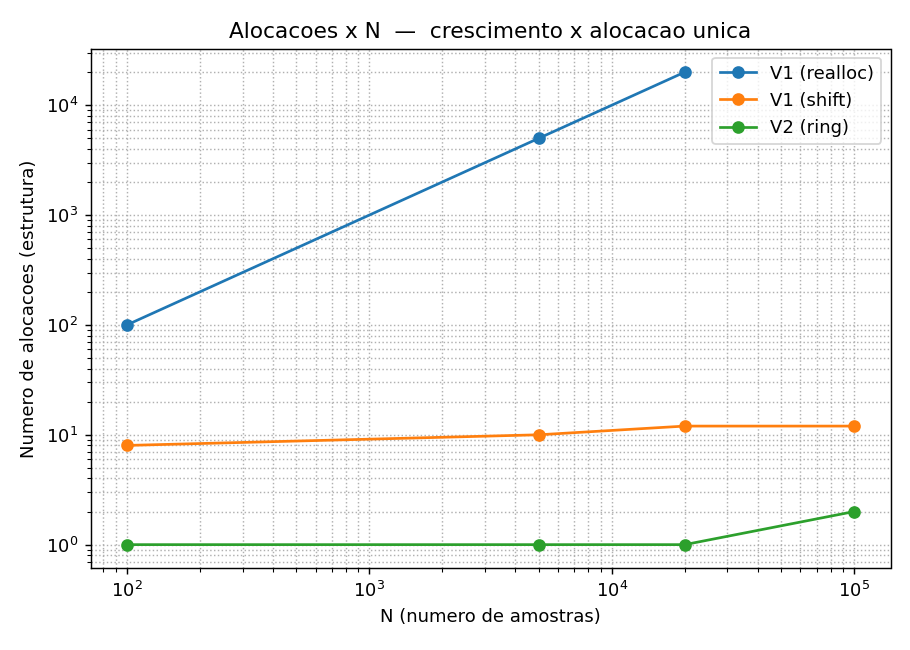
\includegraphics[width=0.78\textwidth]{fig_memoria_vs_N.png}
\caption{Número de alocações atribuídas à estrutura em função de $N$ (log--log).
A alocação única do \texttt{ring} contrasta com o crescimento linear do
\texttt{realloc}.}
\label{fig:mem}
\end{figure}

\begin{figure}[h]
\centering
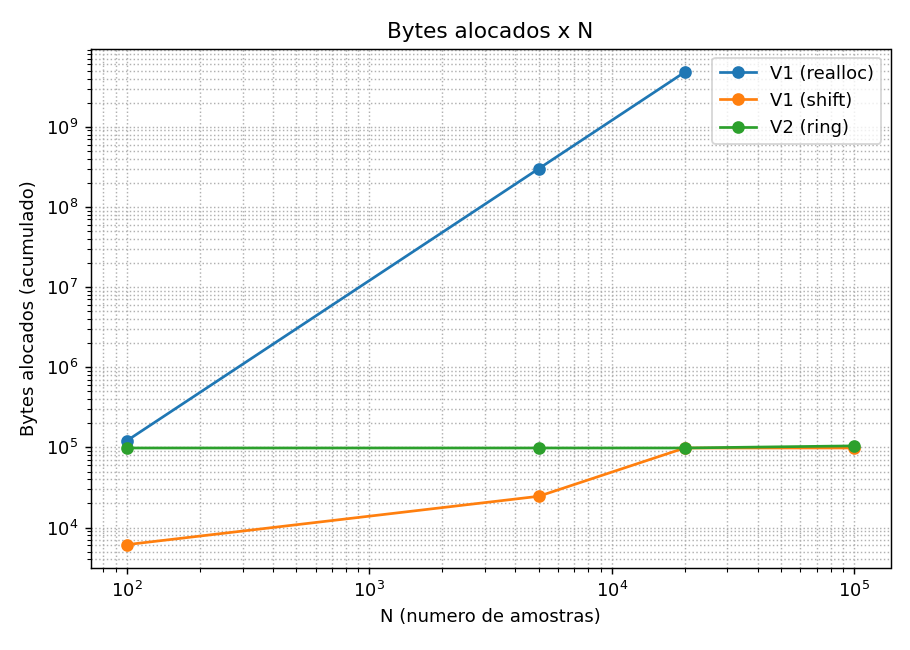
\includegraphics[width=0.78\textwidth]{fig_bytes_vs_N.png}
\caption{Bytes alocados (acumulado) em função de $N$ (log--log).}
\label{fig:bytes}
\end{figure}

\section{Discussão: instabilidade de rede e produtor--consumidor}

O modelo de execução é a diferença central entre as vertentes. A Vertente~1 é
\textbf{síncrona}: captura, insere ($O(n)$) e publica com \texttt{publishSync},
que bloqueia até o \emph{round-trip} da rede; a amostragem \emph{para} durante a
latência. A Vertente~2 é \textbf{assíncrona}: o produtor captura e faz
\texttt{push} $O(1)$ no \texttt{RingBuffer} (nunca bloqueia pela rede), enquanto
um consumidor drena em lote e publica com \texttt{publishAsync}; a sincronização
usa \texttt{mutex} e \texttt{condition\_variable}.

Para simular instabilidade, injeta-se um atraso artificial por publicação
(\texttt{--net-delay-ms}). A Figura~\ref{fig:garg} mostra o efeito sobre a
\emph{taxa de amostragem}: com apenas $1$\,ms de atraso, a Vertente~1 desaba de
$\sim 9 \times 10^5$ para $\sim 64$ amostras/s (a captura fica refém da rede),
enquanto a Vertente~2 mantém a amostragem em $10^5$--$10^6$ amostras/s.

\paragraph{Trade-off da política de overflow.} O desacoplamento tem um custo:
quando o consumidor não acompanha (rede lenta), o \texttt{RingBuffer} satura e
\textbf{sobrescreve as amostras mais antigas}. Ou seja, a Vertente~2 preserva a
\emph{taxa de captura} sacrificando dados antigos, ao passo que a Vertente~1
preserva \emph{todas} as amostras sacrificando a taxa. Para telemetria, em que os
dados recentes valem mais, a política de sobrescrita do buffer circular é a
escolha adequada; o tamanho do buffer dimensiona quanta latência de rede o sistema
absorve antes de começar a descartar.

\begin{figure}[h]
\centering
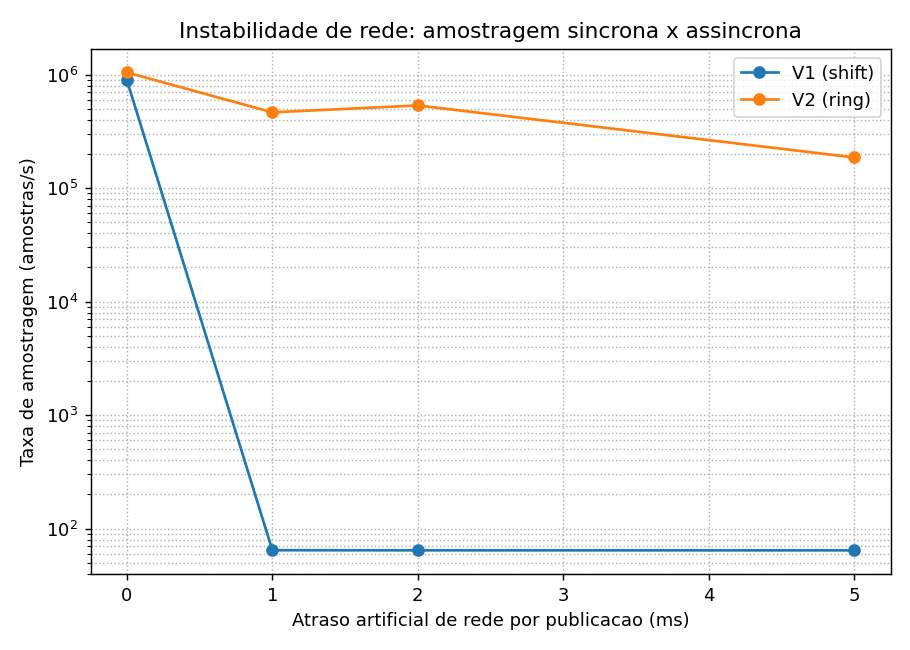
\includegraphics[width=0.78\textwidth]{fig_gargalo.png}
\caption{Taxa de amostragem sob atraso de rede. A vertente síncrona colapsa; a
assíncrona absorve a latência no buffer.}
\label{fig:garg}
\end{figure}

\section{Conclusão}

Os experimentos confirmam, de ponta a ponta, a tese do trabalho. No tempo, a
inserção passa de $O(n)$ (até $O(N^2)$ acumulado na variante \texttt{realloc})
para $O(1)$ com o buffer circular. Na memória, passa-se de $N$ alocações com
crescimento quadrático de bytes para uma \emph{única} alocação de volume
constante. Sob rede instável, o modelo produtor--consumidor com buffer circular
mantém a taxa de amostragem ordens de grandeza acima da abordagem síncrona, ao
preço de uma política de descarte de dados antigos bem definida. O buffer circular
com aritmética modular é, portanto, a estrutura adequada para telemetria de alta
frequência sujeita a latência de rede variável.

\clearpage
\bibliographystyle{plain}
\bibliography{referencias}

\end{document}
